% THIS IS SIGPROC-SP.TEX - VERSION 3.1
% WORKS WITH V3.2SP OF ACM_PROC_ARTICLE-SP.CLS
% APRIL 2009
%
% It is an example file showing how to use the 'acm_proc_article-sp.cls' V3.2SP
% LaTeX2e document class file for Conference Proceedings submissions.
% ----------------------------------------------------------------------------------------------------------------
% This .tex file (and associated .cls V3.2SP) *DOES NOT* produce:
%       1) The Permission Statement
%       2) The Conference (location) Info information
%       3) The Copyright Line with ACM data
%       4) Page numbering
% ---------------------------------------------------------------------------------------------------------------
% It is an example which *does* use the .bib file (from which the .bbl file
% is produced).
% REMEMBER HOWEVER: After having produced the .bbl file,
% and prior to final submission,
% you need to 'insert'  your .bbl file into your source .tex file so as to provide
% ONE 'self-contained' source file.
%
% Questions regarding SIGS should be sent to
% Adrienne Griscti ---> griscti@acm.org
%
% Questions/suggestions regarding the guidelines, .tex and .cls files, etc. to
% Gerald Murray ---> murray@hq.acm.org
%
% For tracking purposes - this is V3.1SP - APRIL 2009

% TODO: Remove these


\newcommand{\todo}[1]{{\textbf{[TODO: #1]}}}
\newcommand{\td}[2]{{\textbf{[TODO: {\it{#1}} #2]}}}

\newcommand{\site}[1]{\texttt{#1}}

\newcommand{\code}[1]{\texttt{#1}}
\newcommand{\quotedcode}[1]{{\vspace{0.5em}\normalfont{\code{#1}\vspace{0.5em}}}}

\newcommand{\iSD}{{\code{includeSubDomains}}}
\newcommand{\ma}{{\code{max-age}}}

\newcommand{\genericsite}{example.com}
\newcommand{\h}{{\site{http://{\allowbreak}\genericsite}}}
\newcommand{\s}{{\site{https://{\allowbreak}\genericsite}}}
\newcommand{\hw}{{\site{http://{\allowbreak}www.\genericsite}}}
\newcommand{\sw}{{\site{https://{\allowbreak}www.\genericsite}}}

\newcommand{\firstsubsectionskip}{{\vspace{1em}}}


\documentclass{acm_proc_article-sp}

\begin{document}

\title{
The State of HSTS Deployment:\\A Survey and Common Pitfalls
}
%
% You need the command \numberofauthors to handle the 'placement
% and alignment' of the authors beneath the title.
%
% For aesthetic reasons, we recommend 'three authors at a time'
% i.e. three 'name/affiliation blocks' be placed beneath the title.
%
% NOTE: You are NOT restricted in how many 'rows' of
% "name/affiliations" may appear. We just ask that you restrict
% the number of 'columns' to three.
%
% Because of the available 'opening page real-estate'
% we ask you to refrain from putting more than six authors
% (two rows with three columns) beneath the article title.
% More than six makes the first-page appear very cluttered indeed.
%
% Use the \alignauthor commands to handle the names
% and affiliations for an 'aesthetic maximum' of six authors.
% Add names, affiliations, addresses for
% the seventh etc. author(s) as the argument for the
% \additionalauthors command.
% These 'additional authors' will be output/set for you
% without further effort on your part as the last section in
% the body of your article BEFORE References or any Appendices.

\numberofauthors{3} %  in this sample file, there are a *total*
% of EIGHT authors. SIX appear on the 'first-page' (for formatting
% reasons) and the remaining two appear in the \additionalauthors section.
%
\author{
% You can go ahead and credit any number of authors here,
% e.g. one 'row of three' or two rows (consisting of one row of three
% and a second row of one, two or three).
%
% The command \alignauthor (no curly braces needed) should
% precede each author name, affiliation/snail-mail address and
% e-mail address. Additionally, tag each line of
% affiliation/address with \affaddr, and tag the
% e-mail address with \email.
%
% 1st. author
\alignauthor
Lucas Garron\\
       \affaddr{Stanford University}\\
       \email{lgarron@cs.stanford.edu}
% 2nd. author
\alignauthor
Andrew Bortz\\
       \affaddr{Dropbox}\\
       \email{abortz@dropbox.com}
\alignauthor
% 3rd. author
Dan Boneh\\
       \affaddr{Stanford University}\\
       \email{dabo@cs.stanford.edu}
}
% There's nothing stopping you putting the seventh, eighth, etc.
% author on the opening page (as the 'third row') but we ask,
% for aesthetic reasons that you place these 'additional authors'
% in the \additional authors block, viz.

\date{October 08, 2013}
% Just remember to make sure that the TOTAL number of authors
% is the number that will appear on the first page PLUS the
% number that will appear in the \additionalauthors section.

\maketitle
\begin{abstract}
HSTS (HTTP Strict Transport Security) has gained significant browser and server adoption since reaching IETF proposed status. However, there are several important deployment challenges. A scan of top websites reveals that many HSTS sites have not properly configured the HSTS header, which still leaves them open to some attacks HSTS is meant to solve. We survey the current state of deployment and describe common mistakes and difficulties with HSTS configuration. We conclude with approaches for properly deploying HSTS as effectively as possible.\end{abstract}

% A category with the (minimum) three required fields
%\category{H.4}{Information Systems Applications}{Miscellaneous}
%A category including the fourth, optional field follows...
%\category{D.2.8}{Software Engineering}{Metrics}[complexity measures, performance measures]

%\terms{Theory}

% \keywords{ACM proceedings, \LaTeX, text tagging} % NOT required for Proceedings


\section{Introduction}
\label{sec:intro}

Although HTTPS can be fairly effective defense against against passive and active attacks, many sites still accept requests over plain HTTP. The HSTS (HTTP Strict Transport Security) browser mechanism helps sites ensure security by avoiding plain HTTP. HSTS is now implemented in three of five major browsers and has seen significant uptake by security-conscious sites -- such as Google, Paypal, Twitter, Stripe, and iCloud.

The core benefit of HSTS is that it allows any host response to specify a {\code{Strict-Transport-Security} header. This creates an entry in the browser that causes all future resource loads from the domain to be sent over HTTPS. If a browser has an HSTS entry for a host, this mitigates a wide variety of attacks, such as eavesdropping, injection/redirection, HTTPS stripping, and DNS spoofing.

However, consider the situation where a user types {\site{\genericsite}} into their browser and is redirected to the canonical domain {\sw}. If the site only sends an HSTS header over {\sw}, future requests without \code{www} will not be secured (e.g. when the user types in the same URL or clicks a link to the unsecured domain). Thus, part of the domain is still suffers from the vulnerabilities HSTS was meant to address.

There are several countermeasures to improve the strength and practicality of HSTS: HSTS provides the {\iSD} directive to protect subdomains of responses. In addition, browsers supporting HSTS ship with a list of preloaded HSTS entries that sites may request to be included in. There are also active efforts for related mechanisms, such as TACK\cite{tack} and other pinning mechanisms. However, these do not intrinsically guard against issues like our redirection example. Related domains and URL canonicalization can easily bypass the intention of HSTS, and deployment for a real-world site can benefit from consideration of browser details like HSTS implementation details and the cache mechanism.

Although some of these issues have been noted as early as 2010\cite{coderrr-blog}, they are not discussed in popular descriptions of HSTS, and many sites still appear to be unaware of them.

\subsection{An Overview of HSTS}

HSTS (HTTP Strict Transport Security) is a browser security mechanism introduced as ForceHTTPS in 2008 by Jackson and Barth\cite{forcehttps} and accepted for the IETF Standards Track in 2012\cite{rfc}. The introduction to RFC 6787 provides a good overview and history of HSTS.

HSTS is a header ({\code{Strict-Transport-Security}}) that a host sends to user agents to request heightened security for a domain. In particular, a conform any browser header that has received an HSTS header from {\h} will will automatically load future all requests to the site from {\s} instead. Thus, HSTS generally touted as a mechanism to ``transform insecure URI references\ldots into secure URI references''. However, it also also enforces strict security in related mechanisms, such as preventing mixed content and ``click-through'' certificate overrides\cite{rfc}.

There are three significantly distinct ways to send the HSTS header; these are described clearly in RFC 6797\cite{rfc}:

{\quotation{\it
The HSTS header field below stipulates that the HSTS Policy is to
remain in effect for one year... and the policy applies only to the domain of the
HSTS Host issuing it:

\quotedcode{
Strict-Transport-Security: max-age=31536000
}}}
{\quotation{\it
The HSTS header field below stipulates that the HSTS Policy is to
remain in effect for approximately six months and that the policy
applies to the domain of the issuing HSTS Host and all of its
subdomains:

\quotedcode{
\noindent Strict-Transport-Security: max-age=15768000 ; includeSubDomains
}}}
{\quotation{\it
The HSTS header field below indicates that the UA must delete the
entire HSTS Policy associated with the HSTS Host that sent the header
field:

\quotedcode{
Strict-Transport-Security: max-age=0
}
}}

The specification also states that the HSTS must only be sent and accepted over HTTPS, and that the {\iSD} directive is ignored for domains when \code{max-age=0}.

In addition, all browsers currently supporting HSTS also ship with a list of known HSTS hosts, called the ``pre-loaded'' / ``preload'' list.

\section{Browser Considerations}
\firstsubsectionskip
\subsection{HSTS Browser Support}

As of September 29, 2013, HSTS is currently supported in the desktop versions of Chrome, Firefox, and Opera. It is not supported in Internet Explorer or Safari.\cite{support}

In addition, the mobile versions of Chrome (iOS and Android) and Firefox (Android) support HSTS like their desktop counterparts\cite{mdn}.

\subsection{Chromium Preload List}

The Chromium project maintains a list of sites in one of its source files\cite{sts-list}. A site owner can request their site to be included in this list to enforce a combination of several browser-side requirements including:

\begin{itemize}
\item \code{force-https} - enables HTTPS for a site by default (without expiration).
\item {\iSD} - same as HSTS.
\item \code{pins} - specific pinned certificates.
\end{itemize}

Google Chrome and Chromium employ this list directly, enforcing the specified security measures.

Chrome considers HSTS to be part of the cache. The ``Empty the cache'' checkbox under ``Clear Browsing data'' wipes stored HSTS values.

\subsection{Opera}

Opera shares the WebKit-derived Blink engine with Chromium, so it exhibits the same HSTS behavior as Chrome.\footnote{Opera originally implemented support in Presto engine\cite{opera}, but Opera is closed-source, and \todo{does not provide explicit documentation about HSTS support since the Blink transition. It behaves like Chrome for preload sites according to the network console.}}

\subsection{Firefox Preload List}

Mozilla ``seeds'' the Firefox preload list by starting with the domains in the Chromium preload list, but performs its own filtering to keep the list fresh and observe the latest host settings. The Chromium list is processed a script\cite{firefox-script} that regularly run \cite{firefox-cron-script} by an automated build bot\cite{firefox-cron}, and the resulting preload list\cite{firefox-list} (along with the list of errors\cite{firefox-errors}) is committed to the \code{mozilla-central} repository.

A site is included in the Firefox preload list if the following hold:

\begin{itemize}
\item It is in the Chromium list (with \code{force-https}).
\item It sends an HSTS header.
\item The \code{max-age} sent is at least $10886400$ ($18$ weeks).
\end{itemize}

Firefox enforces HSTS for all sites in its preload list, which is hard-coded and compiled into the main binary.

The Firefox preload list also includes a boolean flag for \iSD. This flag is set to true if the script recorded {\iSD} in the site's HSTS header (regardless of the Chromium list setting).

The Firefox preload list also includes an expiration time: each script run sets a timeout of $18$ weeks from the time it is run, after which Firefox will ignore it (i.e. sites can use HSTS normally, but the browser will no longer use the preload list to enforce HTTPS on first load for any sites)\cite{firefox-cron-expiration}. Since the release cycle shortens the time HSTS is useful in the browser to significantly less than $18$ weeks, the issue might be addressed in the future, any sites considering HSTS should check current Mozilla policies before selecting a {\ma}.

Firefox considers HSTS to be part of ``Site Preferences'' in its ``Clear Recent History'' feature.

\section{Current Deployment}
\firstsubsectionskip
\subsection{Alexa Top $100000$ Sites}

We automatically surveyed the top $100000$ sites in the Alexa global rankings\cite{alexa} by making \code{GET} requests to four root URLs each:

\begin{itemize}
\item {\h}
\item {\hw}
\item {\s}
\item {\sw}
\end{itemize}

(Where {\site{\genericsite}} represents the domain.)

Although sites may use complicated HSTS mechanisms, we assume that front pages are a sufficient proxy of HSTS behavior. If sites are likely to go for maximum protection and/or simplest configuration, this is a fair assumption.

We recorded which sites:

\begin{itemize}
\item responded over HTTPS at all, either at {\s} or {\sw},
\item how many domains used HSTS with {\ma}$>0$ (and thus had any protection),
\item how may HTTPS sites used {\iSD}, and
\item how many domains used HSTS with a {\ma} of $0$.
\end{itemize}

We only considered HSTS headers that were well-formed and sent over HTTPS on either {\s} or {\sw}. Several technical and financial examples among the top few HSTS sites stand out, but we have not attempted to categorize which kinds of sites use HSTS. The tallies for top sites are summarized in table \ref{table:alexa} and figure \ref{fig:hsts}.

\begin{table}[h!]
\begin{center}
\begin{tabular}{|r|r|r|r|r|}
\hline
$\#$ top sites & HTTPS & HSTS & incl. sub. & \code{max-age=0} \\
\hline
10 & 8 & 1 & 0 & 1 \\
\hline
100 & 76 & 3 & 0 & 2 \\ 
\hline
1000 & 629 & 11 & 3 & 4 \\
\hline
10000 & 5402 & 56 & 11 & 10 \\
\hline
100000 & 46943 & 277 & 66 & 25 \\
\hline
\end{tabular}
\end{center}
\caption{HTTPS adoption vs. adoption of HSTS, HSTS with {\iSD}, and HSTS explicitly disabled.}
\label{table:alexa}
\end{table}%

These numbers were found by using a \code{python} script using the \code{scrapy}\cite{scrapy} library with a current Google Chrome user agent string\footnote{\code{Mozilla/5.0 (Macintosh; Intel Mac OS X 10\_8\_5) AppleWebKit/537.36 (KHTML, like Gecko) Chrome/29.0.1547.76 Safari/537.36}}. All results are from early October 2013. Although we accepted any status code, we only considered initial responses (i.e. no redirects), since a primary goal is to secure the initial landing.

\begin{figure}[h!]
\begin{center}
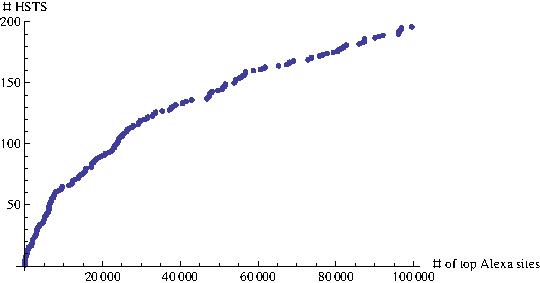
\includegraphics[width=70mm]{alexa_hsts.pdf}
\caption{HSTS adoption among the Alexa top 100000 sites.}
\label{fig:hsts}
\end{center}
\end{figure}

\subsection{The Alexa + Chromium HSTS Sites}

For the rest of this paper, we will discuss sites from two sources:

\begin{itemize}
\item Alexa top $100000$ sites who send a valid HSTS header over HTTPS with {\ma}$ > 0$.
\item Sites from the Chromium HSTS Preload list with \code{force-https} set to \code{true}.
\end{itemize}

Since there is no registry of sites using HSTS (the Chromium preload is closest) and no ``typical'' site using HSTS

\subsection{Common \code{max-age} Settings}

By far the most common {\ma} setting is a static value of $31536000$ seconds, which is roughly one year. This may be because the implementation examples on Wikipedia use this value\cite{wiki}, and it is the {\ma} of two (out of three) examples in RFC 6797\cite{rfc}. The majority of remaining sites are testing HSTS with very low values, ranging from seconds to days, although {\ma} values are as high as $20$ years (\code{twitter.com}).

As an interesting point, nearly every site serving HSTS on both {\s} and {\sw} sends the same {\ma} on both domains.

The {\ma} values group naturally into several buckets, which are displayed in figure \ref{fig:max-age} (including sites with {\ma} $0$ for comparison).

\begin{figure}[h!]
\begin{center}
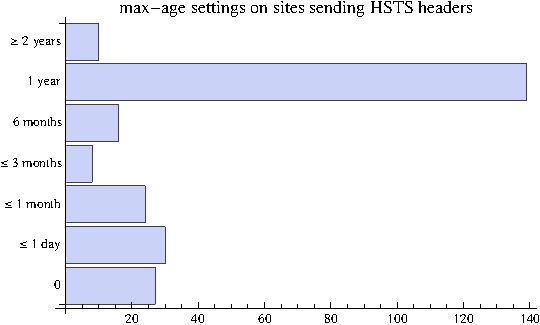
\includegraphics[width=70mm]{max-age.pdf}
\caption{HSTS \code{max-age} settings of sites in the Alexa + Chromium HSTS Sites. (Each site is placed in the highest valid bucket.)}
\label{fig:max-age}
\end{center}
\end{figure}
 

\section{Common Deployment Patterns}

The minimum use of HSTS is to secure a single canonical domain; either {\site{\genericsite}} or {\site{www.\genericsite}}. However, it is usually desirable to do some of the following:

\begin{itemize}
\item Secure all visited (sub)domains (e.g. protect any resource on second load).
\item Secure {\site{\genericsite}} and {\site{www.\genericsite}}.
\item Secure all (sub)domains of {\site{\genericsite}}.
\end{itemize}

Most HSTS sites redirect straight to a canonical URL, adding \code{HSTS} and modifying the presence of \code{www} consistently. However, there is wide variation in redirect schemes and HSTS header. We considered all of the Alexa + Chromium HSTS sites which only redirected to common subdomains of a main domain. There were $409$ of these, including some Chromium sites that do not send HSTS headers.

\subsection{Redirect to {\s}}

A plurality of $78$ sites redirect straight to a final destination of {\s}, where they serve an HSTS header, including $31$ who are subdomains themselves.

Of these, $19$ serve an HSTS header with {\iSD} over {\s}, automatically protecting all subdomains.

$27$ sites did not send an HSTS header over {\sw}, and left it unprotected in all cases.

All but $1$ of these were straight redirects.

\subsection{Redirect to {\sw}}

$37$ sites redirected straight to {\sw}. Although $10$ of them set {\iSD} over {\sw}, only $9$ secured both {\s} and {\sw} at their root URLs -- and only $2$ did both.

$34$ additional sites directed straight to {\sw} but did not allow a valid connection over {\s}. $18$ of these sent {\iSD}.

All but $4$ of these were straight redirects.

\subsection{Redirect to HTTPS}

$24$ sites did not add or remove {\code{www}}. All sites sent an HSTS header over both {\s} and {\sw}. $6$ sent {\iSD} over both, and the rest sent it over neither.

Most of these sent HSTS over both {\s} and {\sw}, with roughly $1/4$ of each using {\iSD}.

All but $4$ of these were straight redirects.

\subsection{Canonical Redirect for HTTP Only}

$23$ sites served either {\s} or {\sw} but consistently redirected plain HTTP requests to {\s}. Another $23$ similarly sent plain HTTP to {\sw} instead, although $13$ of them redirected to {\s} first.

\subsection{Miscellanous}
The remaining sites usually matched the patterns above, with particular anomalies.


\section{Common Mistakes}
% \todo{Or, as Buzzfeed would call it: 3 Ways Your "Secure" Site is Horribly Broken.}
\firstsubsectionskip
\subsection{Permanently Insecure Redirects}

A common pattern is to redirect to {\sw} when the user types \site{\genericsite} into their browser. Assuming the parent domain is not on the preload list, the initial redirect is necessarily insecure on a fresh browser. If the site does not set an HSTS header for {\s}, then this insecure redirect occurs \emph{every time} the user types \site{\genericsite} into their browser.

This is mitigated the browser cache retains an entry for \site{\genericsite}. However, it is undesirable to rely on the cache for such a critical security guarantee, and the protection does not apply for any other pages/resources on {\h} except the specific cached URL.

\subsection{Unprotected Subdomains}

Unless a site sets {\iSD} on {\s}, neither of {\s} or {\sw} automatically set HSTS for each other. Assuming only one of these is visited by a normal user, the other will be unprotected.

\subsection{Accidental HSTS Expiration}

It is reasonable to send an HSTS header at {\h} along with a $30x$ redirect to {\sw}. However, browsers may cache $301$ redirects  aggressively by default. The browser will send {\h} visits directly to {\sw}, without visiting {\s}; thus, the browser will not see another HSTS header for {\s}, and HSTS will eventually expire once the {\ma} is reached. If the {\ma} is updated on the server, the browser will also not see the updated value.

Again, this reduces the security guarantee for HSTS to the cache for known URLs, and will eventually fail to protect other resources.

\subsection{Clerical Mistakes}

$30\%$ of HSTS sites in our survey also send an HSTS header over {\h} or {\hw}. While an RFC-conforming browser is required to ignore this, RFC 6797\cite{rfc} also states that:

\begin{quotation}\it
An HSTS Host MUST NOT include the STS header field in HTTP responses conveyed over non-secure transport.
\end{quotation}

Sending the header over plain HTTP suggests an unfamiliarity with HSTS, apathy towards the specification, or inadequate control over redirect configuration.

In our scans, we also encountered various occasional mistakes, such as using a comma instead of a semicolon, sending an integer value without \code{max-age=}, including the \code{must-revalidate} directive (thus resembling a cache-control header), or removing the hyphen from \code{max-age}. A few sites, including \code{paypal.com}, also send two HSTS headers in the same request.

\section{Issues with Improving HSTS Configuration}
\firstsubsectionskip
\subsection{Canonical Subdomain}

If the canonical domain for a site is {\sw}, the user may rarely load a page/resource from {\s}. This makes it more difficult to secure a fresh visit to {\s}, should the user visit it directly later. It also fails to protect any other subdomains.

\subsection{Implications of \iSD}
\label{includeSubDomains-issues}

In practice, using {\iSD} may mot be straightforward at the top-level ({\s}) of an existing site because there is at least one subdomain that may break over HSTS. Possibilities for this include:

\begin{itemize}
\item Insecure resources will fail to load and break pages that worked over HTTPS without HSTS.
\item Such a large change is usually accompanied by increasing the scope of secure redirects (``\emph{if} we're going to do it, we may as well do it all at once''), which may break certain clients that rely on plain HTTP.\item The server for a subdomain is not configured to use HTTPS.
\item It may be impractical/expensive/risky to furnish every subdomain server with a valid CA-signed certificate.
\item The browser will prevent the user from using self-signed certificates for any subdomains.
\item The browser will enforce HTTPS for all subdomains even if there are other security measures in place (such as local testing or gating for a corporate network) that would otherwise allow the continued use of plain HTTP.
\end{itemize}

While it is worthwhile to address these issues and move towards more robust solutions that can operate under HSTS with \iSD, any site should be aware of these issues before considering HSTS a free panacea.

\section{Best Practice}

With regard to HSTS, a site should operate under the threat model that an attacker can run a man-in-the-middle attack over plain HTTP for any (sub)domain of the site, e.g. by exposing a victim to spoofed DNS entries. However, the attacker cannot intercept or modify valid HTTPS traffic over any of these subdomains.

Thus, it is desirable to protect as many subdomains as possible, as early as possible, by registering HSTS for them in the browser.

\subsection{Ideal Practice}


The strongest protection is to

\begin{itemize}
\item redirect every resource to HTTPS immediately
\end{itemize}

and serve well-formed  HSTS header:

\begin{itemize}
\item with every HTTPS request,
\item with a long \code{max-age} (18 weeks minimum, $1$ year recommended), and
\item with {\iSD}.
\end{itemize}

To be fully correct, the site must also:

\begin{itemize}
\item never send an HSTS header over plain HTTP.
\end{itemize}

This protects all future requests to the site or any of its subdomains. If the canonical site is {\s}, any requests to the site will automatically extend the expiration date (including for subdomains).

In addition, once a site is committed to HSTS, it should:
\begin{itemize}
\item be included in the browser preload lists.
\end{itemize}

Any security-conscious site should strive to all of take these steps, if possible. In case this is initially impractical

\subsection{Send an HSTS header whenever possible}

It is advisable to send an HSTS header on any request sent from a (sub)domain only intended to be accessed over HTTPS. This ensures that HSTS is enabled on every subdomain as early as possible, without depending on other sub/superdomains.

In addition, every visit extends the expiration of HSTS.

\subsection{Send the most secure settings possible}

Every site should aim to ramp up its \code{max-age} as high as possible (at least to the popular default of $6$ or $12$ months).

As advocated in section $14.4$ of RFC 6797\cite{rfc}, a site should aim to send \code{includeSubdomains} whenever possible. Although section \ref{includeSubDomains-issues} discusses issues with {\iSD} for {\s}, it is usually safe to send {\iSD} on any particular subdomain, including {\sw}.

\subsection{Redirect Immediately and Securely}

Unless legacy use cases require plain HTTP support, every request should be redirected to HTTPS (using a $30x$ status) before any content is served.

Any redirect served over HTTPS should include an HSTS header, to ensure that the redirect is fully secured in the future.

A site should redirect HTTP requests to the HTTPS version the request before performing other canonicalization steps like adding/removing \code{www}. This ensures that HSTS will be applied to future redirects on the same domain.

In case all the redirect URLS and final destinations of a site are protected using {\iSD} at the destination, a two-hop redirect and a separate HSTS setting for the redirect (sub)domain may seem redundant. However, the first redirect will be eliminated once HSTS in place, and continues to protect the redirect in case {\iSD} needs to be removed.

\subsection{Securing {\s} from a subdomain}

If most pages are served from a subdomain like {\sw}, securing the entire domain requires an additional step. A simple solution is to make a request to an uncached HSTS-serving resource on {\s}, such as a $1$-pixel \code{<img>}. This is best done using a cache-control header, but simple cache-busting tricks work equally well.

This uncached-resource approach works in all current HSTS browsers. In case a site would like to minimize resource fetches, the particular HSTS resource can:
\begin{itemize}
\item send a short-lived \code{cache-control} header for the resource instead, and/or
\item be configured not redirect from {\s} to {\sw}.
\end{itemize}

Such a solution is being used successfully in practice, e.g. by \site{https://www.icloud.com}.

\subsection{Ensure that incoming visits are secure}

Although a site should serve a plain HTTP request once if it is received, it is useful to protect them from ever doing so, by making sure they are likely to visit over HTTPS first (and are protected from future insecure visits if HSTS is enabled).

Once a site is committed to HTTPS, it should ensure that all links on the website are updated to HTTPS (or protocol-relative URLs) and that automatically generated links (e.g. shortened URLs, ``copy link'' buttons, API-generated links) are generated with \code{https://}. This will help ensure that future incoming visits are secured immediately.


\section{Conclusion}

We described the current state of HSTS in the specification and browser implementation. Based on this, we surveyed top sites and found a few of them send an HSTS header, but many of them do not secure as many of their (sub)domains as they should -- leaving them open to many attacks that HSTS was meant to mitigate. In particular found that canonicalization redirects often stay insecure even if HSTS is used at the final page. We briefly discussed that sites should be aware of when using {\iSD}, and concluded with concrete suggestions to improve HSTS deployment. These suggestions mostly center around selecting the most secure options available, and ensuring that the browser receives them for the desired domain -- either during a redirect or using a resource load on the final destination.

These results remind us that HSTS, while effective, should not be treated like snake oil. Sites must be aware of HSTS details, and we hope this paper provides many of the details helpful for making the correct choices about initial and continued deployment.

We note that most of the issues stem from the fact that HSTS can only protect the current domain and not subdomains. Our survey shows that sites are likely to end up with unintentional security weaknesses given the currently available information. Thus, we hope that future work will either address related domains at the specification level, or that the issues and solutions identified in this paper are clearly available to sites considering HSTS -- leading to a more secure web.

\bibliographystyle{abbrv}
\bibliography{hsts}  % sigproc.bib is the name of the Bibliography in this 

\end{document}
